\dev{Emile Martinez}{}

\section{Gestion par la machine (Terminale)}

\subsection{Motivation}

Lorsque vous utilisez votre PC, vous éxécutez des dizaines de programmes «en même temps» (lecture de courriel, taper au clavier, écouter de la musique...). Pourtant, votre PC a un nombre limité de processeurs. Comment fonctionne cette illusion ?

\subsection{Exécution concurrente}

\begin{definition}
	Un processus est un programme en cours d'exécution sur un ordinateur. Il dispose d'une zone mémoire en RAM. Le système d'exécution identifie les processus grâce à un numéro unique appelé PID.
\end{definition}

\begin{definition}[Exécution concurrente]
	Deux processus s'exécutent en concurrence si les intervalles entre leur commencement et leur fin respective sont non disjoints.
\end{definition}

\begin{principe}[Fonctionnement de l'exécution concurrente]
	Le système d'exploitation peut interrompre un processus en cours pour exécuter du code qui lui est propre. Il peut alors, à intervalles réguliers, décider à quelle tâche en cours il rend la main. 
	
	Le rôle de l'ordonnanceur est de choisir le prochain processus à exécuter parmi une liste de processus candidats. 
\end{principe}

\begin{center}
	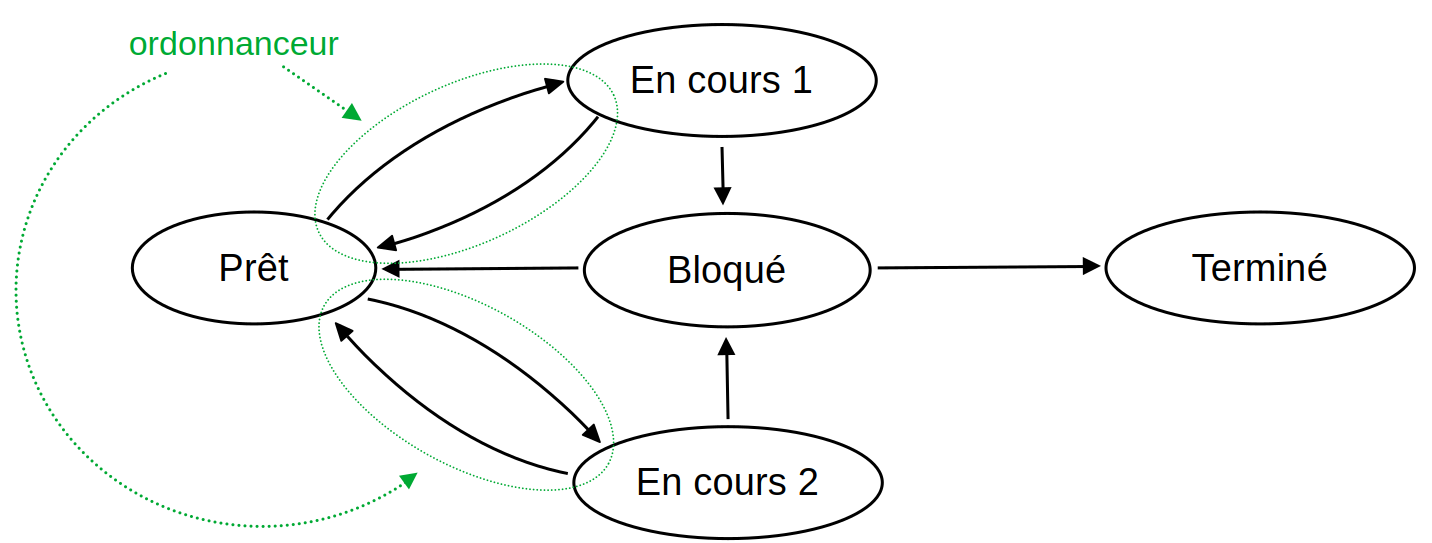
\includegraphics[width=0.9\linewidth]{lecon/17-ordonnancement/graphe_etat.png}\\
	Cycle de vie d'un processus
\end{center}

\subsection{L'ordonnanceur}

On peut vouloir des garanties sur la manière dont l'ordonnanceur choisit ses tâches.

\begin{definition}
	On dit qu'il y a absence de famines (ou vivacité) si aucun processus n'attend indéfiniment.
\end{definition}

\begin{definition}
	On dit qu'il y a équité si aucun processus n'est favorisé.
\end{definition}

\begin{algo}[Algorithme du tourniquet]
	L'ordonnanceur définit un intervalle de temps $\tau$. 
	
	Il place les processus en attente dans une file selon leur ordre d'arrivée (PAPS).
	
	Tant que la file est non vide, il en sort le premier et l’exécute durant tau. Si besoin, il le ré-insert en queue de file.
\end{algo}

\begin{example} Exemple d'exécution sur 3 processus et un seul processeur\\
	\begin{center}
		
		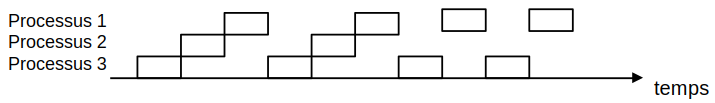
\includegraphics[width=0.8\linewidth]{lecon/18-fil/tourniquet.png}
	\end{center}
\end{example}

\begin{proposition}
	L'algorithme du tourniquet garantie l'équité et l'absence de famine.
\end{proposition}

\begin{rem}
	Certains processus étant plus importants que d'autres, on peut adapter le temps tau à chaque processus, en fonction de leur priorité.
\end{rem}

\subsection{Commande unix de gestion de processus}

\noindent \begin{minipage}{0.3\linewidth}
	\begin{lstlisting}
$ ps
	\end{lstlisting}
\end{minipage}\quad\begin{minipage}{0.6\linewidth}
	permet d'afficher les processus en cours, et leur taux d'occupation du processeur et de la mémoire. 
\end{minipage}\\

\noindent \begin{minipage}{0.3\linewidth}
	\begin{lstlisting}
$kill 6555
	\end{lstlisting}
\end{minipage}\quad\begin{minipage}{0.6\linewidth}
	envoie un  signal de terminaison au processus de PID 6555. (Pour une application graphique, c'est ce que fait la croix rouge)
\end{minipage}\\

\noindent \begin{minipage}{0.3\linewidth}
	\begin{lstlisting}
$top
	\end{lstlisting}
\end{minipage}\quad\begin{minipage}{0.6\linewidth}
	affiche la liste des processus prêts et en cours.
\end{minipage}

\section{Gestion par l'utilisateur (prépa)}

\subsection{Motivation}

\begin{definition}
	Un fil d'exécution (thread en anglais) est un sous processus qui partage la mémoire avec les autres fils du processus.
\end{definition}

\begin{impl}
	En C, un programme peut lancer d'autres fils d'exécution, de type \texttt{pthread\_t} et que l'on lance avec la fonction \texttt{pthread\_create}
\end{impl}

\begin{idee}
	On peut alors gérer des choses en parallèle
\end{idee}

\begin{example}
	\label{18-somme-para} \normalfont
	Somme parallélisée d'un tableau T de taille 2m.\\\\
	\begin{minipage}{0.45\linewidth}
		Fil 1 :
		\begin{lstlisting}[style=CStyle]
for(int i = 0; i < m; i++){
	int s = res + T[2*i];
	res = s;  }\end{lstlisting}
	\end{minipage} \quad
	\begin{minipage}{0.45\linewidth}
		Fil 2:
	\begin{lstlisting}[style=CStyle]
for(int i = 0; i < m; i++){
	int s = res + T[2*i + 1];
	res = s;  }\end{lstlisting}
	\end{minipage}\\
	On peut donc aller deux fois plus vite.
	
	\paragraph{Question :} Que se passe-t-il sur l'exécution F1:1 $\to$ F2:2 $\to$ F1:3 $\to$ F2:3 ?
\end{example}

\subsection{Les verrous}

\begin{definition}
	Le problème de l'exclusion mutuelle consiste à garantir que deux fils d'exécution n'essaieront pas d'exécuter simultanément un morceau de code prédéfini.
\end{definition}

\begin{example}
	Les lignes 2 et 3 pour les fils 1 et 2 de l'exemple \ref{18-somme-para}.
\end{example}

\begin{definition}
	Un verrou (ou mutex) est une structure de données permettant deux opérations : \begin{itemize}
		\item \texttt{prendre()} : appel bloquant qui demande l'accès au verrou
		\item \texttt{rendre()} : appel qui libère le verrou
	\end{itemize}
\end{definition}

\begin{proposition}
	Une implémentation efficace des verrous devrait garantir l'exclusion mutuelle, l'absence de famine et l'équité.
\end{proposition}

\begin{algo}
	L'algorithme de Peterson propose une implémentation des verrous pour deux fils vérifiant ces propriétés.
\end{algo}

\paragraph{Développement :} Présentation de l'algorithme de Peterson et preuve de fonctionnement.

Extension à n fils d'exécution :
\begin{algo} \normalfont Algorithme de la boulangerie de Lamport\\
\begin{minipage}{0.6\linewidth}
	\begin{lstlisting}[style=CStyle]   
void prendre(int i ){
	Acq[i] = 1;
	int t = 0;
	for(int j = 0; j < n; j++)
		t = MAX(t, num[j]);
	num[i] = t + 1;
	Acq[i] = 0;
	
	for(int j = 0; j < n; j++){
		while (acq[j] == 1);
		while (num[j] == 1 && (num[j] < num[i] 
			|| (num[j] == num[i] && j < i)) );
	}
}

void rendre(int i){
	num[i] = 0;
}\end{lstlisting}
\end{minipage}
\begin{minipage}{0.25\linewidth}
	$\begin{array}{l}
	\left. \begin{array}{c} \\ \\ \\ \\ \\ \end{array} \right\} \begin{array}{c} \\ \\ \text{Obtenir un} \\\text{numéro} \\ \\ \end{array} \\
	\\
	\left. \begin{array}{c} \\ \\ \\ \\ \end{array} \right\} \begin{array}{c} \\ \text{Attendre son} \\\text{tour pour prendre} \\ \text{le verrou} \\ \end{array}
	\\ \\ \\ \\ \\
	\end{array}
	$
\end{minipage}
\end{algo}

\paragraph{Analogie :} On prend un ticket dans une boulangerie, et on attend que ce soit notre tour.

\begin{rem}
	L'attente ici est active (on effectue des opérations quand on attend)
\end{rem}

\begin{impl}
	\normalfont
	En C : Les verrous sont disponibles dans la bibliothèque pthread. \begin{itemize}[label=]
		\item type : \texttt{pthread\_mutex\_t}
		\item initialisation : \texttt{pthread\_mutex\_init(pthread\_mutex\_t *m, NULL)}
		\item prendre : \texttt{pthread\_mutex\_lock(pthread\_mutex\_t *m)}
		\item rendre : \texttt{pthread\_mutex\_unlock(pthread\_mutex\_t *m)}
	\end{itemize}
\end{impl}

\begin{rem}
	Une mauvaise utilisation des verrous peut créer des interblocages.
\end{rem}

\begin{example} \enspace\\ \normalfont
	\begin{minipage}{0.3\linewidth}
	Fil 1 :
	\begin{lstlisting}[style=CStyle]
prendre(m1);
prendre(m2);\end{lstlisting}
\end{minipage} \quad
\begin{minipage}{0.3\linewidth}
	Fil 2:
	\begin{lstlisting}[style=CStyle]
prendre(m2);
prendre(m1);\end{lstlisting}
\end{minipage}
\end{example}

\begin{com}
	Ici on ne prend pas un exemple plus gros, comme le dîner des philosophes, car ici on ne veut pas s'étendre sur ça, simplement faire une ouverture, et mentionner le problème.
\end{com}

\section{Les sémaphores}

\paragraph{Analogie :} Tableau des clés d'un hôtel

\begin{definition}
	Un sémaphore est un compteur qui propose les opérations suivantes :
	\begin{itemize}
		\item Initialiser à une valeur entière
		\item décrémenter : appel bloquant, décrémente le compteur s'il est positif, attend qu'il le soit sinon
		\item incrémenter : incrémente le compteur. S'il devient positif, cela libère un fil si un attendait
	\end{itemize} 
\end{definition}

\begin{appl}
	Limiter l'accès à une ressource à $n$ fils.
\end{appl}

\begin{com}
	On ne s’appesantit pas sur cette application au vu de sa complexité. Donc même si c'est l'application la plus directe et que dans un vrai cours, on aurait peut-être ici un petit programme l'utilisant pour illustrer le concept, on se concentre nous sur des choses plus importantes.
\end{com}

\begin{rem}
	On peut implémenter un verrou par un sémaphore initialisé à 1.
\end{rem}

\begin{impl}
	Les sémaphores sont disponibles dans la bibliothèque semaphore.h.
	\begin{itemize}
		\item type : \texttt{sem\_t}
		\item initialisation : \texttt{sem\_init}
		\item décrémenter : \texttt{sem\_wait}
		\item incrémenter : \texttt{sem\_post}
	\end{itemize}
\end{impl}

\begin{proposition}
	L'implémentation des sémaphore est faites (normalement) sans attente active.
\end{proposition}

\begin{appl}[Problème du rendez-vous]
	On a p fils qui doivent se synchroniser. Chacun travaillant en deux phases. Dans la première phase, tous les fils sont indépendants et peuvent s’exécuter simultanément. La deuxième phase d'un fil ne peut débuter que si tous les fils ont terminé la première.\\
	
	On peut résoudre ce problème à l'aide de sémaphore.
\end{appl}

\paragraph{Développement :} Solutions aux problèmes du rendez-vous

\begin{appl}[Producteur / Consommateur] \normalfont
	On dispose d'un tampon de taille N, et on a deux types de fils : \begin{itemize}
		\item des producteurs qui produisent des ressources et les stockent dans le tampon
		\item des consommateurs qui consomment les données produites (consommer une donnée libère son emplacement)
	\end{itemize}
	
	Pour que la donnée consommée soit la plus vieille, le tampon est circulaire :
	\begin{center}
		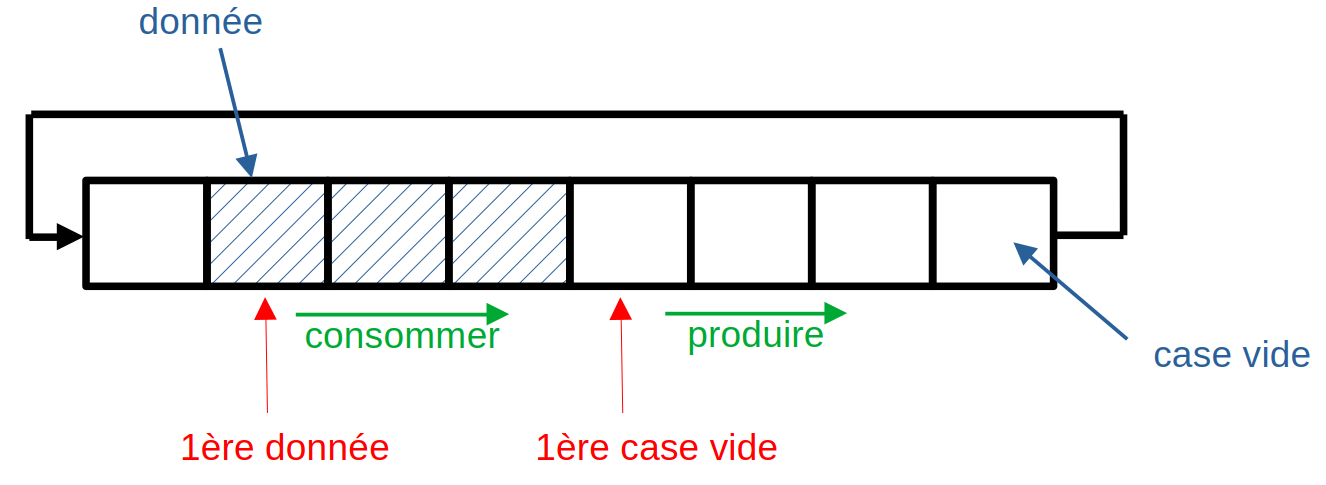
\includegraphics[width=0.7\linewidth]{lecon/18-fil/prod-cons.png}
	\end{center}
	
	\paragraph{Problème :} \begin{itemize}
		\item l'accès au tampon est partagé
		\item les consommateurs doivent attendre qu'une place soir produite
		\item les producteurs doivent attendre que de la place soit libérée dans le tampon.
	\end{itemize}
	
	\paragraph{Solution :} On utilise un sémaphore indiquant le nombre données disponibles et un le nombre de cases disponibles.
	
	\begin{lstlisting}[style=CStyle]
sem_t mutex, vide, plein;
sem_init(&mutex, 0, 1);
sem_init(&vide, 0, N);
sem_init(&plein, 0, 0);\end{lstlisting}

\begin{minipage}{0.45\textwidth}
		Producteur :
		\begin{lstlisting}[style=Cstyle]
int item;
while(1){
	item = produire_item()
	// On attend un place
	sem_wait(&vide);
	sem_wait(&mutex);
	insert_item(item);
	sem_post(&mutex);
	// On la remplie
	sem_post(&plein);
}\end{lstlisting}
	\end{minipage}\qquad
	\begin{minipage}{0.45\textwidth}
		Consommateur :
		\begin{lstlisting}[style=Cstyle]
int item;
while(1){
	// On attend un element
	sem_wait(&plein);
	sem_wait(&mutex);
	item = remove_item();
	sem_post(&mutex);
	// On libere une place
	sem_post(&vide);
	consomer_item(item);
}\end{lstlisting}
	\end{minipage}
	
\end{appl}

\begin{com}
	Par manque de place, on peut moins s'étendre et ne pas écrire l'algorithme, se contenter de dire qu'on a un sémaphore qui compte les places vides et un les places pleines. (et éventuellement virer le dessin)
\end{com}

\begin{rem}
	On peut implémenter un sémaphore par de l'attente active et des verrous. Donc naturellement, ce qu'apporte souvent les sémaphores, par rapport au verrou, c'est moins d'attente active.
\end{rem}

\begin{com}
	Cette remarque, car si on a des élèves un peu rapide, il pourrait trouver assez facilement des solutions n'utilisant que des verrous, et donc se poserait la question de la pertinence des sémaphores dans ce contexte. L'intérêt des sémaphores vient alors de la suppression de l'attente active.
\end{com}

\begin{com}
	On ne mentionne pas tous les problèmes possibles liés aux sémpahores, car ici dans cette leçon on doit parler de plein d'aspects différents. On se limite alors à en expliquer le fonctionnement global et à les illustrer.
\end{com}